% book of game theory exercises
% nicola frosi
% starting date 05-06-2024

\documentclass[a4paper, twoside, openany]{book}

\usepackage[utf8]{inputenc}
\usepackage[T1]{fontenc}
\usepackage[english]{babel}

\usepackage[margin=2.5 cm]{geometry}

\usepackage{float}
\usepackage{rotating}


\usepackage{amsmath}
\usepackage{amsfonts}
\usepackage{amssymb}
\usepackage{amsthm}

\DeclareMathOperator*{\argmax}{arg\,max}
\DeclareMathOperator*{\argmin}{arg\,min}

\usepackage{tikz}
\usetikzlibrary{arrows.meta, calc, quotes}

\newcommand{\norm}[1]{\left\lVert#1\right\rVert}
\newcommand{\esssup}{\operatornamewithlimits{ess\,sup}}

\title{\textbf{\huge{\textit{A collection of Game Theory exercises}}}}

\begin{document}
\maketitle
\section*{Exercise $1$}
Two people are employed in a joint project. If every person $i=1,2$ spends an amount of resources $x_i$, where $0 \leq x_i \leq 1$, incurring a cost $k_i(x_i)$, the project will have a revenue of $f(x_1, x_2)$. The revenue is equally divided by the two persons, without considering the resources employed by each person.
\begin{itemize}
\item write the payoff function of each player;
\item formulate this problem as a strategic game and determine the possible Nash equilibria in the cases: 
				\begin{enumerate}
				\item $f(x_1, x_2) = 3 x_1 x_2 \qquad \textrm{and} \qquad k_i(x_i) = x_i^1 \qquad \textrm{for} \qquad i=1,2$;
				\item $f(x_1, x_2) = 4 x_1 x_2 \qquad \textrm{and} \qquad k_1(x_1) = x_1, \qquad k_2(x_2) = \frac{2}{3}x_2$.
				\end{enumerate}
\end{itemize}
In the prevoius cases can we deduce a priori that a Nash equilibrium exists?
\section*{Solution}
\textbf{case a)} \par
i) proceed:
$$f(x_1, x_2) = 3x_1 x_2,$$
the proceed for every single person is:
$$f_i(x_1, x_2) = \frac{3}{2} x_1 x_2.$$
The payoff functions are:
$$u_1(x_1, x_2) = \frac{3}{2}x_1 x_2 - x_1^2$$
$$u_2(x_1, x_2) = \frac{3}{2}x_1 x_2 - x_2^2.$$
The strategic game $(A_1 \times A_2, (u_1, u_2))$ is such that:
$$A_1 = A_2 = [0, 1]$$
$$u_1(x_1, x_2) = \frac{3}{2}x_1 x_2 - x_1^2$$
$$u_2(x_1, x_2) = \frac{3}{2}x_1 x_2 - x_2^2.$$
We now need to calculate the best reply:
$$BR_i:= A_{-i} \rightarrow A_i \qquad \forall i = 1, 2, \cdots, n,$$
that is
$$BR_1:= A_2 \rightarrow A_1 \qquad \forall x_2 \in [0, 1],$$
given by
$$BR_1(x_2) = \argmax_{x_1 \in [0,1]} u_1(x_1, x_2) = \argmax_{x_1 \in [0,1]} \frac{3}{2} x_1 x_2 - x_1^2 = \argmax_{x_1 \in [0, 1]} (\frac{3}{2}x_2 - x_1)x_1.$$
We have that
$$\frac{\partial u_1(x_1, x_2)}{\partial x_1} = \frac{3}{2}x_2 - 2 x_1 = 0$$
for
$$x_1 = \frac{3}{4}x_2,$$
so that
$$BR_1(x_2) = \frac{3}{4}x_2.$$
The best reply for the player two is:
$$BR_2:= A_1 \rightarrow A_2 \qquad \forall x_1 \in [0, 1]$$
given by
$$BR_1(x_1) = \argmax_{x_2 \in [0, 1]} u_2(x_1, x_2) = \argmax_{x_2 \in [0, 1]} \frac{3}{2}x_1 x_2 - x_2^2$$
so that
$$\frac{\partial u_2(x_1, x_2)}{\partial x_2} = \frac{3}{2}x_1 - x_2 = 0$$
for
$$x_2 = \frac{3}{4} x_1,$$
so that
$$BR_2(x_1) = \frac{3}{4}x_1.$$
\begin{figure}[!ht]
\begin{center}
\begin{tikzpicture}[scale=5.0]
\draw[->] (-0.2,0)--(1.5,0) node[below]{$x_1$};   
\draw[->] (0,-0.2)--(0,1.5)  node[left]{$x_2$};
\draw[dashed] (1.0,-0.2)--(1.0,1.2);
\draw[dashed] (-0.2,1.0)--(1.2,1.0);
\path
(0,0) node[below left]{$0$};
\path
(1.0,0) node[below right]{$1.0$};
\path
(0.0,1.0) node[below left]{$1.0$};
\foreach \i in {0,0.1, 0.2,...,1.0} \draw (\i,-0.02)--(\i,0.02);
\draw[green, domain=0.:1.0, samples=100, variable=\x] plot ({\x}, {3./4*\x});
\draw[orange, domain=0.:3./4, samples=100, variable=\x] plot ({\x}, {4./3*\x});
\path
(0.5,0.7) node[left]{$B_1$};
\path
(0.8,0.4) node[left]{$B_2$};
\filldraw [red] (0,0) circle (1pt) node[above left] (2.1) {$N.E.$};
\end{tikzpicture}
\end{center}
\end{figure}
We can also solve the following system:
$$\begin{cases}
	x_1 = \frac{3}{4}x_2 \\
	x_2 = \frac{3}{4}x_1
   \end{cases} \implies
   \begin{cases}
   x_1 = 0 \\
   x_2 = 0
   \end{cases}$$
$$(0,0) \qquad \textrm{is the unique Nash Equilibrium}.$$
\textbf{case b)} \par  
i) Payoff functions:
$$f(x_1, x_2) = 4 x_1 x_2,$$
then for each player the proceeds is
$$f_i(x_1, x_2) = 2x_1 x_2,$$
so that the payoff functions are:
$$u_1(x_1, x_2) = 2 x_1 x_2 - x_1$$
$$u_2(x_1, x_2) = 2x_1 x_2 - \frac{2}{3}x_1.$$
ii) Now we consider the two players strategic game $(A_1 \times A_2, (u_1, u_2))$ such that
$$A_1 = A_2 = [0, 1]$$
$$u_1(x_1, x_2) = 2 x_1 x_2 - x_1$$
$$u_2(x_1, x_2) = 2 x_1 x_2 - \frac{2}{3}x_2.$$
Now we can consider the Best Reply
$$BR_i:= A_{-i} \rightarrow A_i \qquad \forall i = 1, 2, \cdots, n$$
that are
$$BR_1:= A_2 \rightarrow A_1$$
$$BR_2:= A_1 \rightarrow A_2.$$ 
From the definition we have
$$BR_i(a_{-i}) = \{ a_i \in A_i \qquad \textrm{s.t.} \qquad u_i(a_{-i}, a_i) \geq u_i(a_{-i}, \hat{a}_i) \qquad \forall \hat{a}_i \in A_i \}$$
$$ = \argmax_{\hat{a}_i \in A_i} u_i(a_{-i}, \hat{a}_i)$$
$$BR_1(x_2) = \argmax_{x_1 \in [0,1]} (2x_1 - 1)x_1 = \begin{cases}
														\{ 0 \} \qquad \textrm{if} \qquad x_2 < \frac{1}{2} \\
														[0, 1] \qquad \textrm{if} \qquad x_2 = \frac{1}{2}\\
														\{ 1 \} \qquad \textrm{if} \qquad x_2 > \frac{1}{2}
													 \end{cases}$$
													 
\begin{figure}[!ht]
\begin{center}
\begin{tikzpicture}[scale=5.0]
\draw[->] (-0.2,0)--(1.5,0) node[below]{$x_1$};   
\draw[->] (0,-0.2)--(0,1.5)  node[left]{$x_2$};
\draw[dashed] (1.0,-0.2)--(1.0,1.2);
\draw[dashed] (-0.2,1.0)--(1.2,1.0);
\path
(0,0) node[below left]{$0$};
\path
(1.0,0) node[below right]{$1.0$};
\path
(0.0,1.0) node[below left]{$1.0$};
\foreach \i in {0,0.1, 0.2,...,1.0} \draw (\i,-0.02)--(\i,0.02);
\draw[blue, line width = 1.5] (0,0.0)--(0,0.5);
\draw[blue, line width = 1.5, domain=0.:1., samples=100, variable=\x] plot ({\x}, {0.5});
\draw[blue, line width = 1.5] (1.,0.5)--(1.,1.);
\path
(0.5,0.7) node[left]{$B_1$};
\end{tikzpicture}
\end{center}
\end{figure}			
$$BR_2 := A_1 \rightarrow A_2 \qquad \forall x_1 \in [0, 1]$$
$$BR_2(x_1) = \argmax_{x_2 \in [0, 1]} (2x_1 -\frac{2}{3})x_2 = \begin{cases}
																\{ 0 \} \qquad \textrm{if} \qquad x_1 < \frac{1}{3} \\
																[0, 1] \qquad \textrm{if} \qquad x_1 = \frac{1}{3}\\
																\{ 1 \} \qquad \textrm{if} \qquad x_1 > \frac{1}{3}
                                                                \end{cases}$$
                                   
\begin{figure}[!ht]
\begin{center}
\begin{tikzpicture}[scale=5.0]
\draw[->] (-0.2,0)--(1.5,0) node[below]{$x_1$};   
\draw[->] (0,-0.2)--(0,1.5)  node[left]{$x_2$};
\draw[dashed] (1.0,-0.2)--(1.0,1.2);
\draw[dashed] (-0.2,1.0)--(1.2,1.0);
\path
(0,0) node[below left]{$0$};
\path
(1.0,0) node[below right]{$1.0$};
\path
(0.0,1.0) node[below left]{$1.0$};
\foreach \i in {0,0.1, 0.2,...,1.0} \draw (\i,-0.02)--(\i,0.02);
\draw[green, line width = 1.5] (0,0.0)--(1./3,0.0);
\draw[green, line width = 1.5] (1./3,0.)--(1./3,1.);
\draw[green, line width = 1.5, domain=1./3:1., samples=100, variable=\x] plot ({\x}, {1.0});
\path
(0.5,0.7) node[left]{$B_2$};
\end{tikzpicture}
\end{center}
\end{figure}	
From the definition 
$$a^{\star} \in A \qquad \textrm{is a Nash Equilibrium}$$
$$\textrm{iff}$$
$$a_i^{\star} \in BR_i(a_{-i}^{\star} \qquad \forall i$$
\begin{figure}[!ht]
\begin{center}
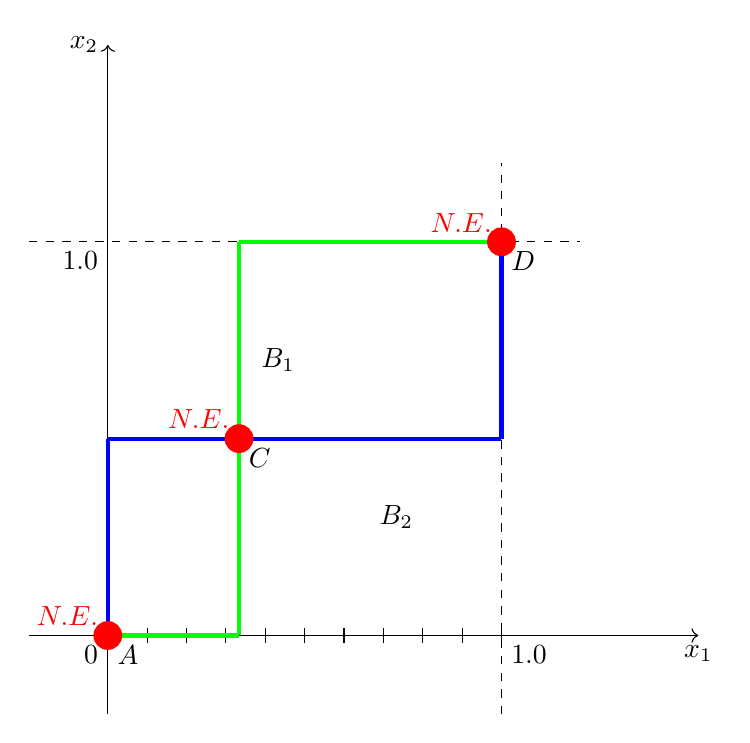
\begin{tikzpicture}[scale=5.0]
\draw[->] (-0.2,0)--(1.5,0) node[below]{$x_1$};   
\draw[->] (0,-0.2)--(0,1.5)  node[left]{$x_2$};
\draw[dashed] (1.0,-0.2)--(1.0,1.2);
\draw[dashed] (-0.2,1.0)--(1.2,1.0);
\path
(0,0) node[below left]{$0$};
\path
(1.0,0) node[below right]{$1.0$};
\path
(0.0,1.0) node[below left]{$1.0$};
\foreach \i in {0,0.1, 0.2,...,1.0} \draw (\i,-0.02)--(\i,0.02);
\draw[green, line width = 1.5] (0,0.0)--(1./3,0.0);
\draw[green, line width = 1.5] (1./3,0.)--(1./3,1.);
\draw[green, line width = 1.5, domain=1./3:1., samples=100, variable=\x] plot ({\x}, {1.0});
\draw[blue, line width = 1.5] (0,0.0)--(0,0.5);
\draw[blue, line width = 1.5, domain=0.:1., samples=100, variable=\x] plot ({\x}, {0.5});
\draw[blue, line width = 1.5] (1.,0.5)--(1.,1.);
\path
(0.5,0.7) node[left]{$B_1$};
\path
(0.8,0.3) node[left]{$B_2$};
\filldraw [red] (0,0) circle (1pt) node[above left] (2.1) {$N.E.$};
\filldraw [red] (1./3,1./2) circle (1pt) node[above left] (2.1) {$N.E.$};
\filldraw [red] (1.,1.) circle (1pt) node[above left] (2.1) {$N.E.$};
\path
(0.,0.) node[below right]{$A$};
\path
(1./3,1./2) node[below right]{$C$};
\path
(1.,1.) node[below right]{$D$};
\end{tikzpicture}
\end{center}
\end{figure}	
The Nash Equilibrium are
$$B_1 \cap B_2 = \{ A, C, D \}$$
where
$$A = (0,0)$$
$$C = (1./3, 1./2)$$
$$D = (1., 1.)$$
The functions $u_i: A_1 \times A_2 \rightarrow \mathbb{R}$ are continuous. The map $x_1 \mapsto u_1(x_1, x_2)$ with $x_2 \in A$ fixed is linear in $x_1$ and so it is concave. The same for the map $x_2 \mapsto u_2(x_1, x_2)$ with $x_1 \in A$ fixed. Then the Nash Theorem guarantees the existence of at least a Nash Equilibrium.

		
\end{document}